\chapter{Conclusions and Future Developments}
\label{ch:chapter_nine}%

This final chapter presents the concluding remarks of this thesis, highlighting its contributions to autonomous multimodal motion control. Additionally, potential future work is discussed, focusing on necessary improvements in both hardware and decision/control algorithms.

\section{Research Contributions}
\label{sec:contribution}

This thesis's achievements contribute to establishing a research foundation on multilimbed robots. 
A formal definition of these robots, never provided in the literature, has been proposed, and a new research topic has been discussed. The base manipulability ellipsoid makes possible a comprehensive analysis of complex multilimbed systems configurations, and the definition of dexterity-aware motion tasks, as proved by the grasshopper analysis. 
Furthermore, this thesis contributes to the development of multimodal multilimbed robots, which is a promising field of research to achieve autonomy in unstructured environments. The transformable module analyzed here and the stable locomotion transition algorithm defined are enough modular to be extended for any multilimbed robotic system and terrain condition. 

Additionally, the work conducted in this thesis would be beneficial in future works on LIMBERO-GRIEEL at the SRL, and the transformation algorithm will be tested on a renewed version of the robot (described in the next section). The preliminary simulation experiments and the lessons learned from the simulator set-up are fundamental in the next research steps, and the same holds for the new simulation environment. In conclusion, the MATLAB code used for the kinematic analysis and manipulability analysis of multilimbed robots is \href{https://github.com/AlePuglisi/limbed-robot-control}{open source}, for any researcher to contribute on the extension of this theory. 

\section{Future Work}
\label{sec:future}

In previous chapters, when limitations and opportunities were evident in the analysis, insights on the required components and hardware improvements were presented. 
Here, the most relevant for generic multimodal robots and LIMBERO-GRIEEL are reported, and organized as: hardware, global planning, and local planning/controller design. The meaning of each of these components has been defined previously, and here it is briefly summarized at the beginning of each class summary. First, the novel base manipulability ellipsoid theory is discussed.  

\subsection{Novel Multi-Limbed Robots Manipulability Ellipsoid}
\label{sec:BME_future}
The BME theory introduced in this research is a powerful tool to define task-oriented dexterous posture for multilimbed robots, and also to analyze the mechanical structure performance in the design phase.

Currently, this index considers only kinematic, and as noticed in Chapter \ref{ch:chapter_three}, In some configurations, such as base at the limit vertical height, the results are not reliable. 

The misleading results in some non-dexterous configurations are related to how the overall contribution of the limbs is combined in the differential kinematic model. 
For this reason, additional scaling will be based on mechanical joint limits or constraints of the overall closed kinematic chain.   

Finally, future extensions similar to the one existing for robot manipulators will be considered, such as the Dynamic manipulability ellipsoid\cite{AsadaDynamicManipulability}\cite{Siciliano}, and Polytope space \cite{PolytopesManipulability}\cite{velocityWorkspacePolytope}. 

In conclusion, with this approach, the manipulability and dexterity are analyzed based on the robot's configuration, and integrating stability in a novel criterion can guarantee further improvements in the evaluation of multi-limb robot performances. 
For example, an interesting approach consist in the evaluation of a climbing robot's performance by combining the ellipsoid region with the stability polyhedron\cite{GIA_polyedron} by mapping those in the same space.


\subsection{Hardware}
\label{sec:Hardware}
This section considers all the aspects of the robot hardware, such as mechanical design, actuators, and sensors.

From the observations of Chapter \ref{ch:chapter_seven}, and the quantitative results and limitations described in Chapter \ref{ch:chapter_eigth}, the required hardware improvements of the systems are clear. 

The limitations of the hardware experiments motivate the SRL to improve the mechanical design of the LIMBERO-GRIEEL limb. 
In the new version, the following re-designs are integrated into the completely new version of the GRIEEL module, as represented in Fig.\ref{fig:newGrieel}:
\begin{itemize}
    \setlength\itemsep{-0.7em} 
    \item New \textbf{finger joint actuation} mechanism. This new design is based on the BMX bicycle gyro brake system, allowing the repositioning of the locking motor on the limb's root. This re-design reduces significantly the weight of GRIEEL, solving one of its main criticalities. Furthermore, transformation time is reduced, improving the performance of the proposed locomotion transition algorithm. 
    \item \textbf{Removed wristV} joint. The joint configuration described in Chapter\ref{ch:chapter_four} has 3 DOFs, with the wristV joint controlling the pitch angle. The same task-space variable of the EE was already controlled by the T2E joint. Furthermore, as noticed in the previous chapter, the gravitational load on that joint servomotor was critical, and torque overload often caused a failure. 
    For those reasons, the wirstV joint has been removed from the actuation system. 
    \item New \textbf{fingers structure}. To increase the contact area of the wheel for better performance and stability, the fingers have been redesigned with longer grousers and a different mechanical structure.  
    \item New \textbf{joint motors}. In the new version, more powerful DYNAMIXELs motors have been employed. 
\end{itemize}

\begin{figure}[H]
    \centering
    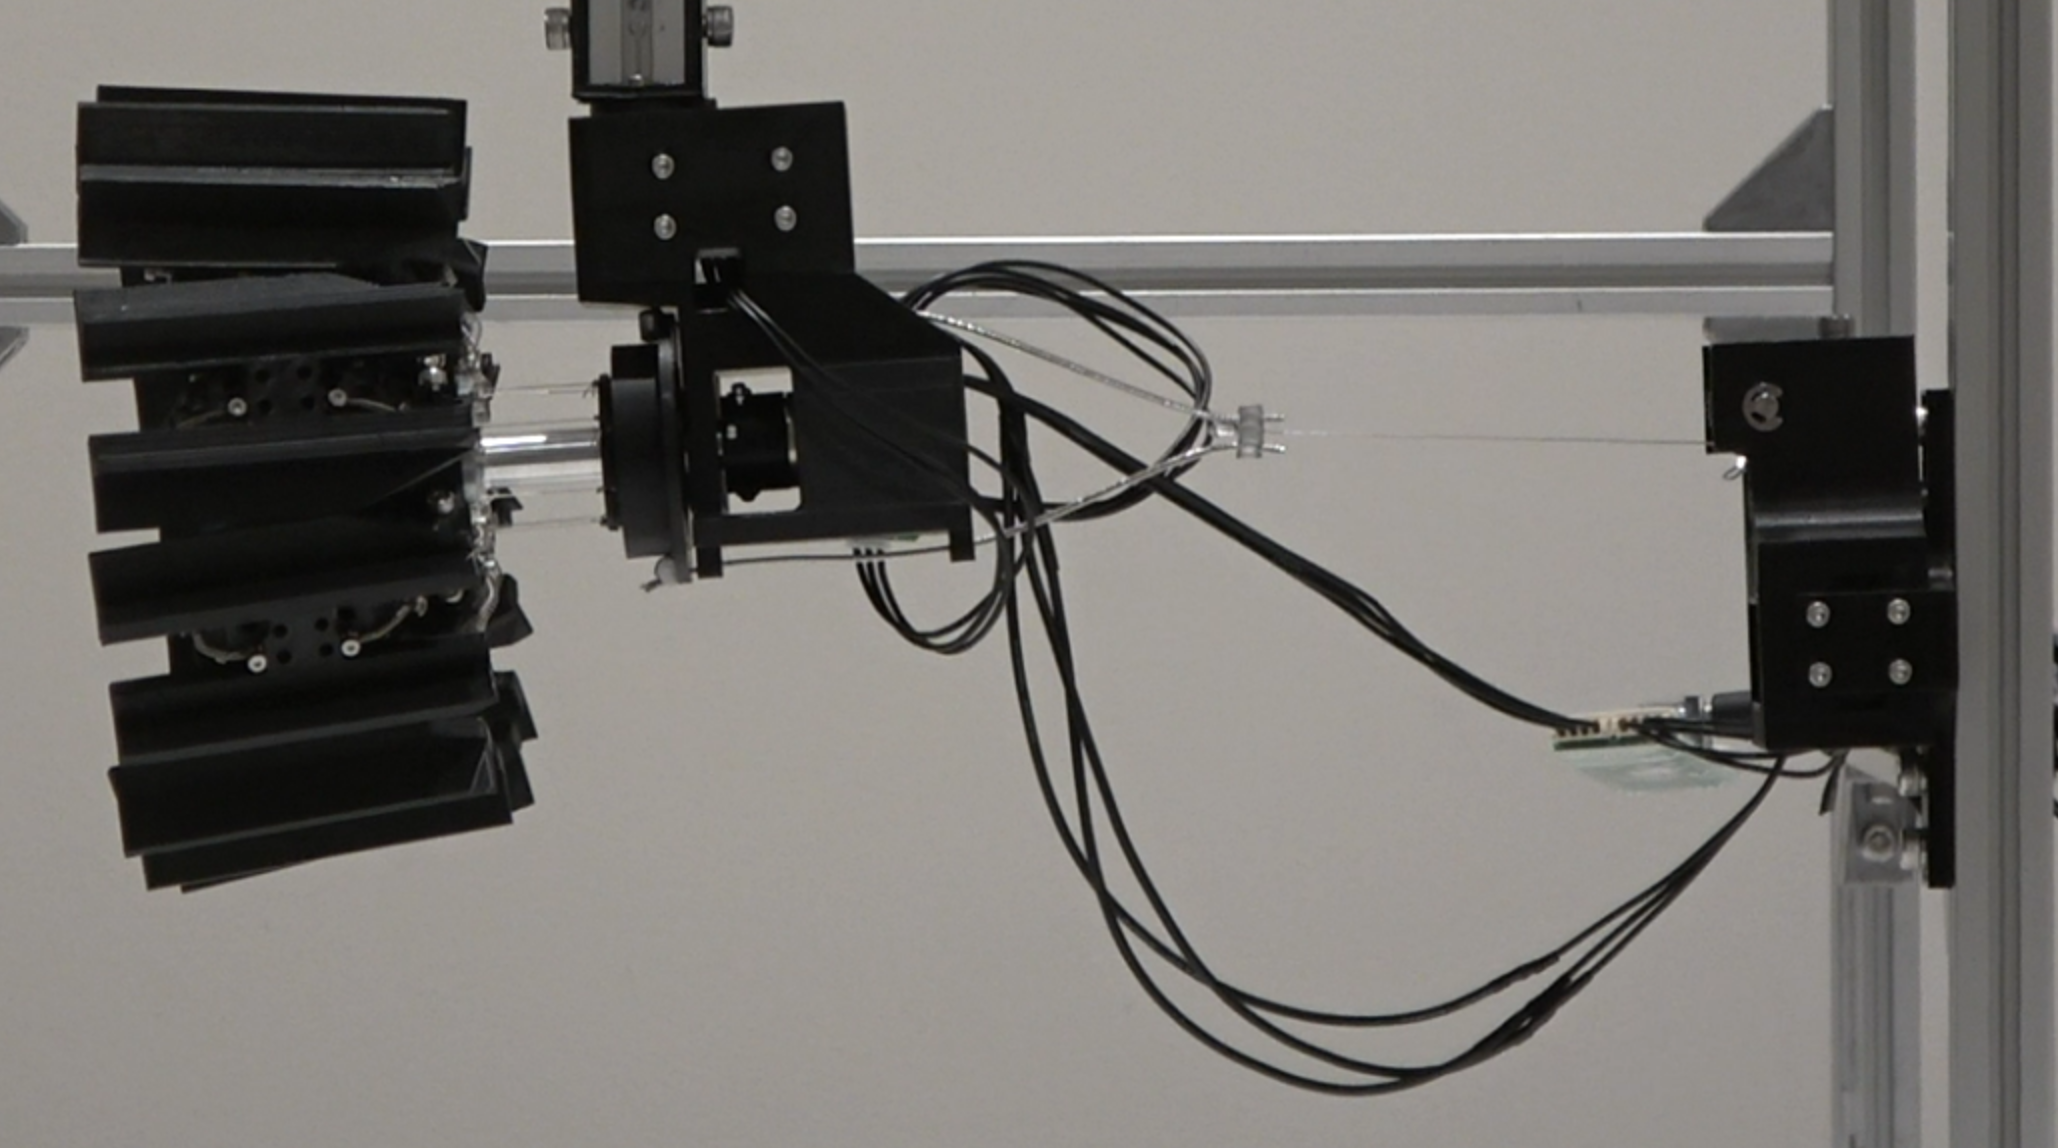
\includegraphics[width=0.5\textwidth]{Images/img_ch9/GRIEELv2.png}
    \caption{New GRIEEL mechanism, separate locking motor}
    \label{fig:newGrieel}
\end{figure}

LIMBERO's limb was originally designed for a lightweight spine gripper used for climbing, however, the employment of the transformable module makes the system multifunctional. 
As the experiments proved, a more reliable limb mechanical structure is required to account for higher EE payloads and inertial effects. 

In the new mechanical design of the limb, the femur has been completely remodeled with a closed kinematic chain mechanism and a more efficient transmission system. 
With this redesign, the limitations of the shoulder and elbow joints are accounted for, but additional kinematic complexity is integrated with the closed chain. 
The new limb is represented in Fig.\ref{fig:newLimb}, and the overall robot LIMBERO-GRIEELv2 in Fig.\ref{fig:newrobot}.

\begin{figure}[H]
    \centering
    \subfloat[Payload test in wheel mode\label{fig:contact}]{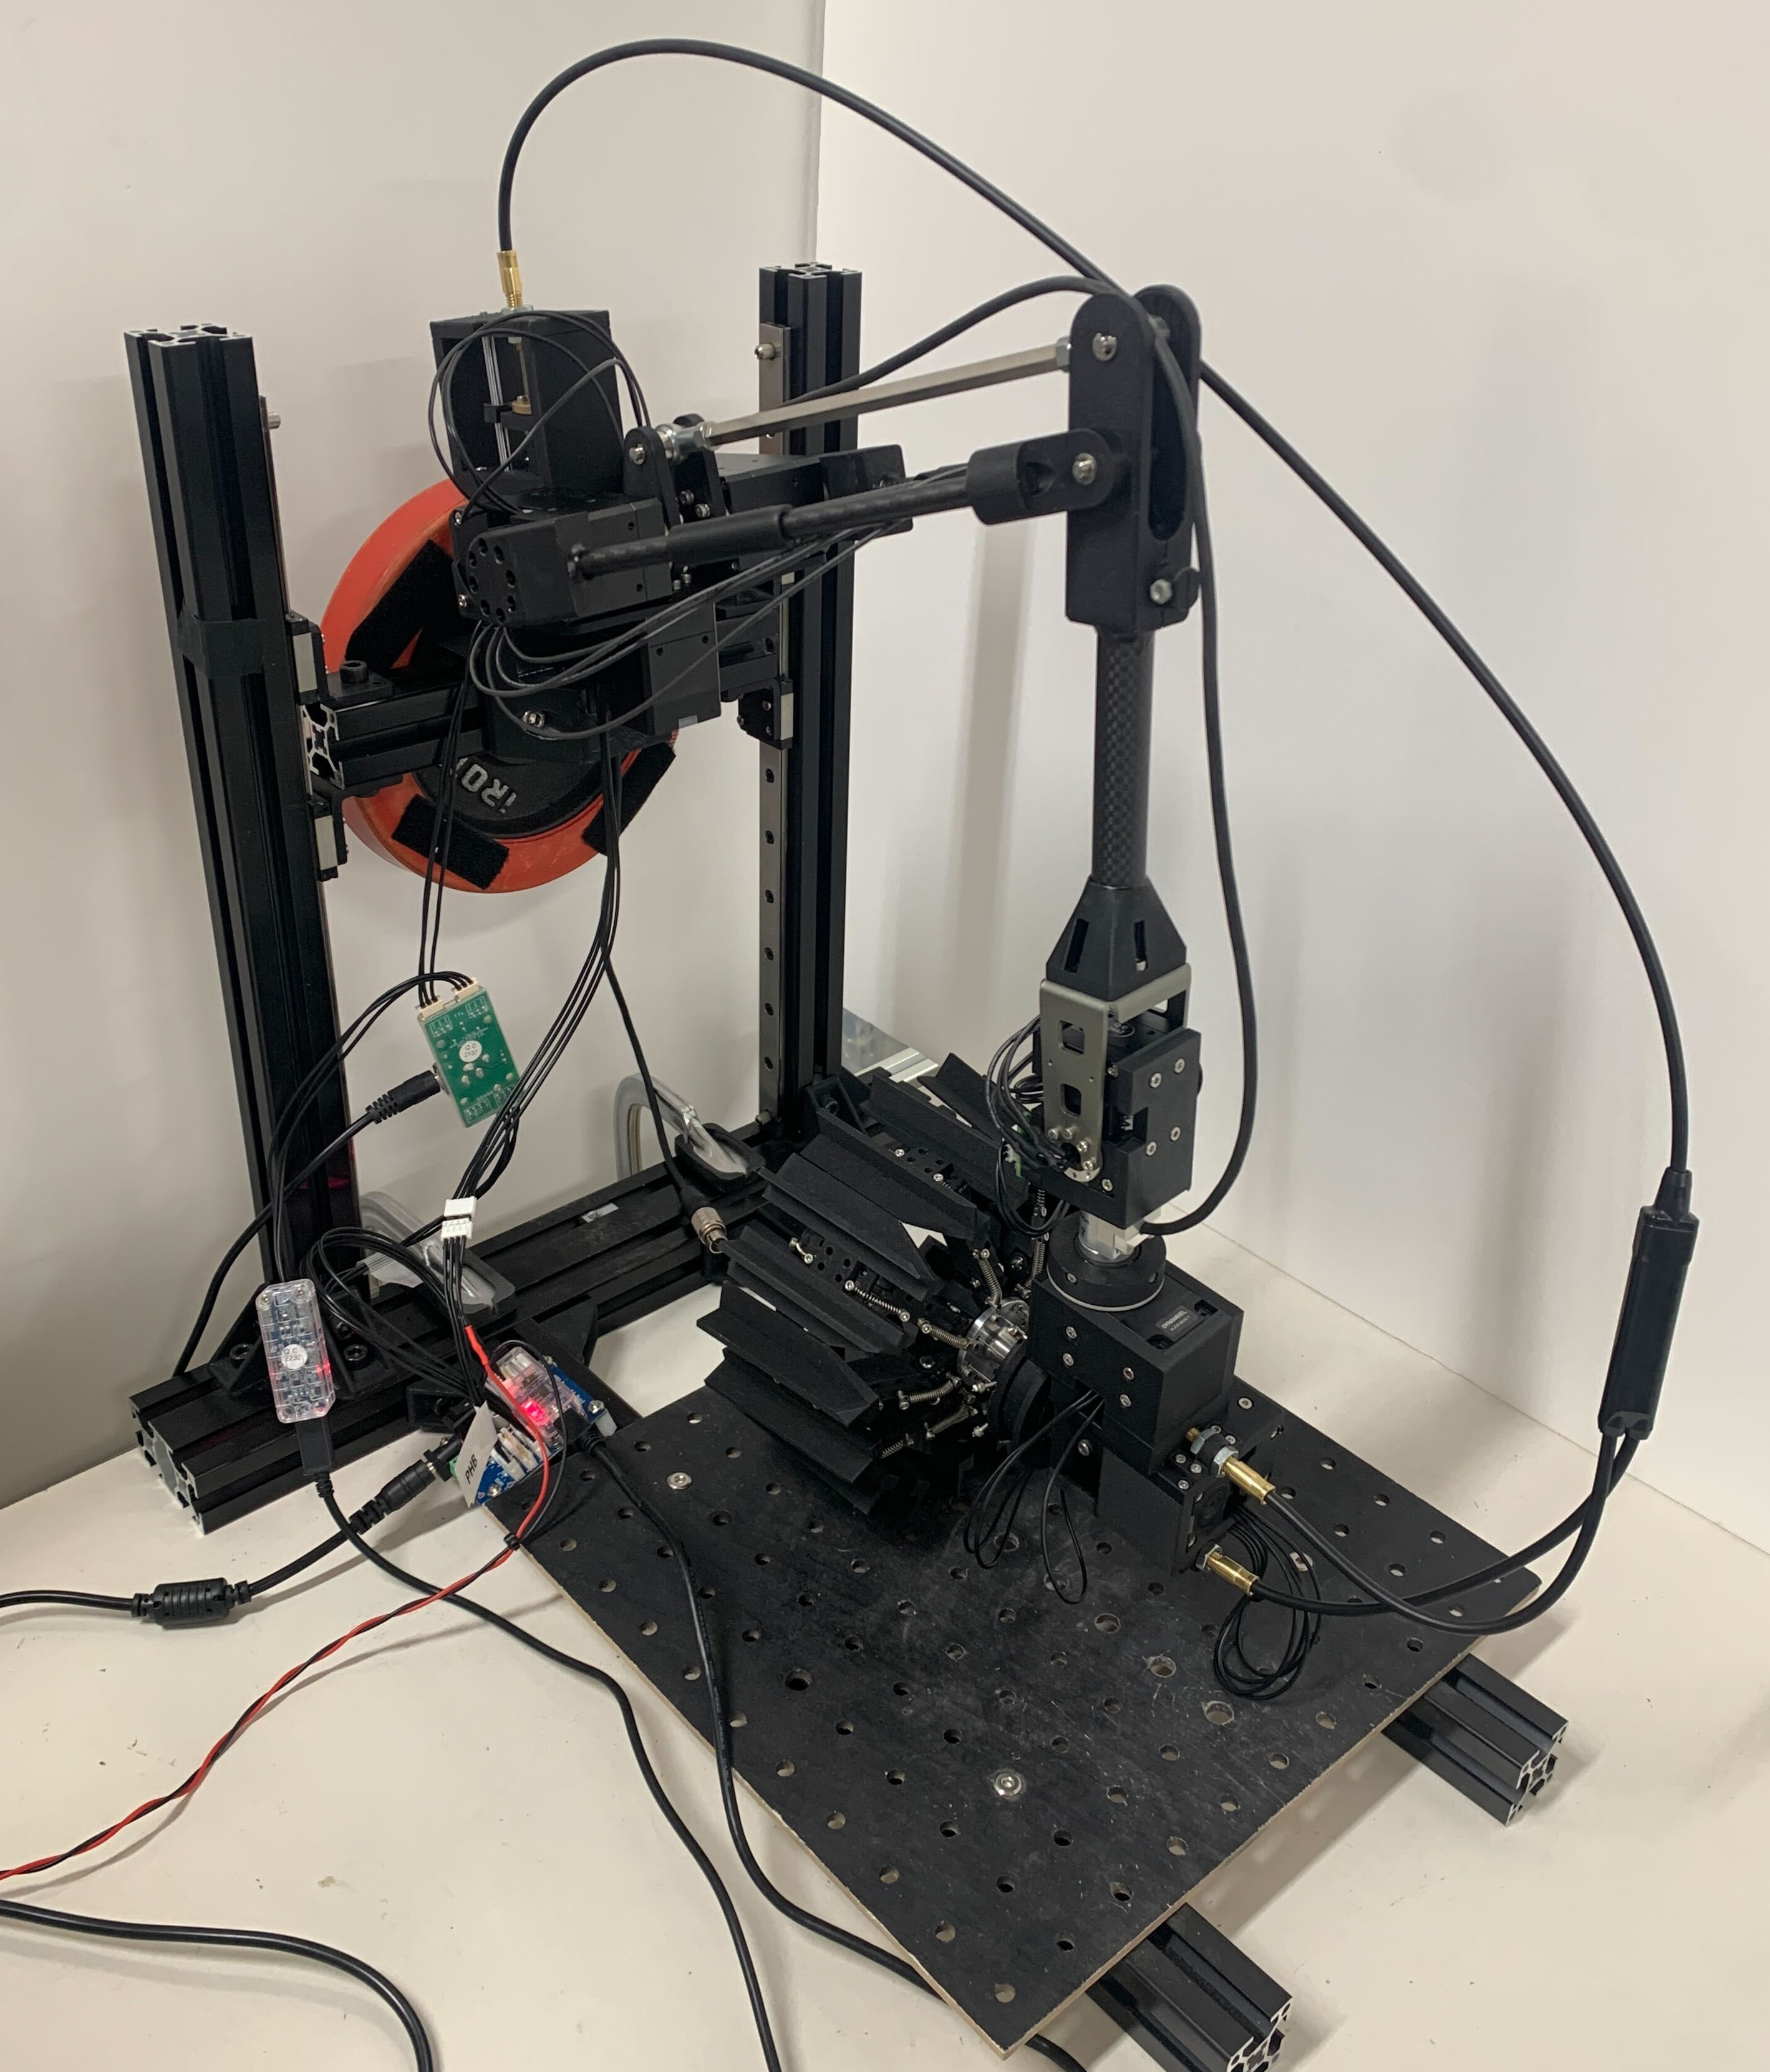
\includegraphics[width=0.35\textwidth]{Images/img_ch9/limb_hw.jpg}} \quad 
    \subfloat[New limb CAD\label{fig:not_contact}]{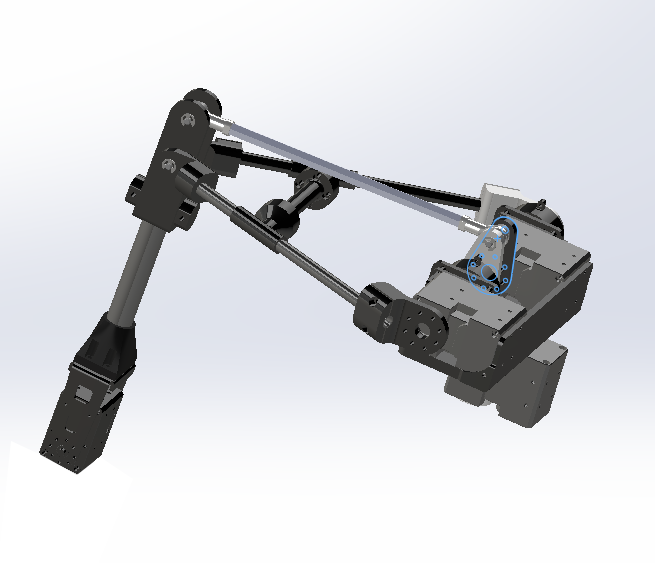
\includegraphics[width=0.45\textwidth]{Images/img_ch9/limb_scheme.png}} 
    \caption[New limb design]{New limb design}
    \label{fig:newLimb}
\end{figure}
\begin{figure}[H]
    \centering
    \subfloat[Gripper modes\label{fig:gripperv2}]{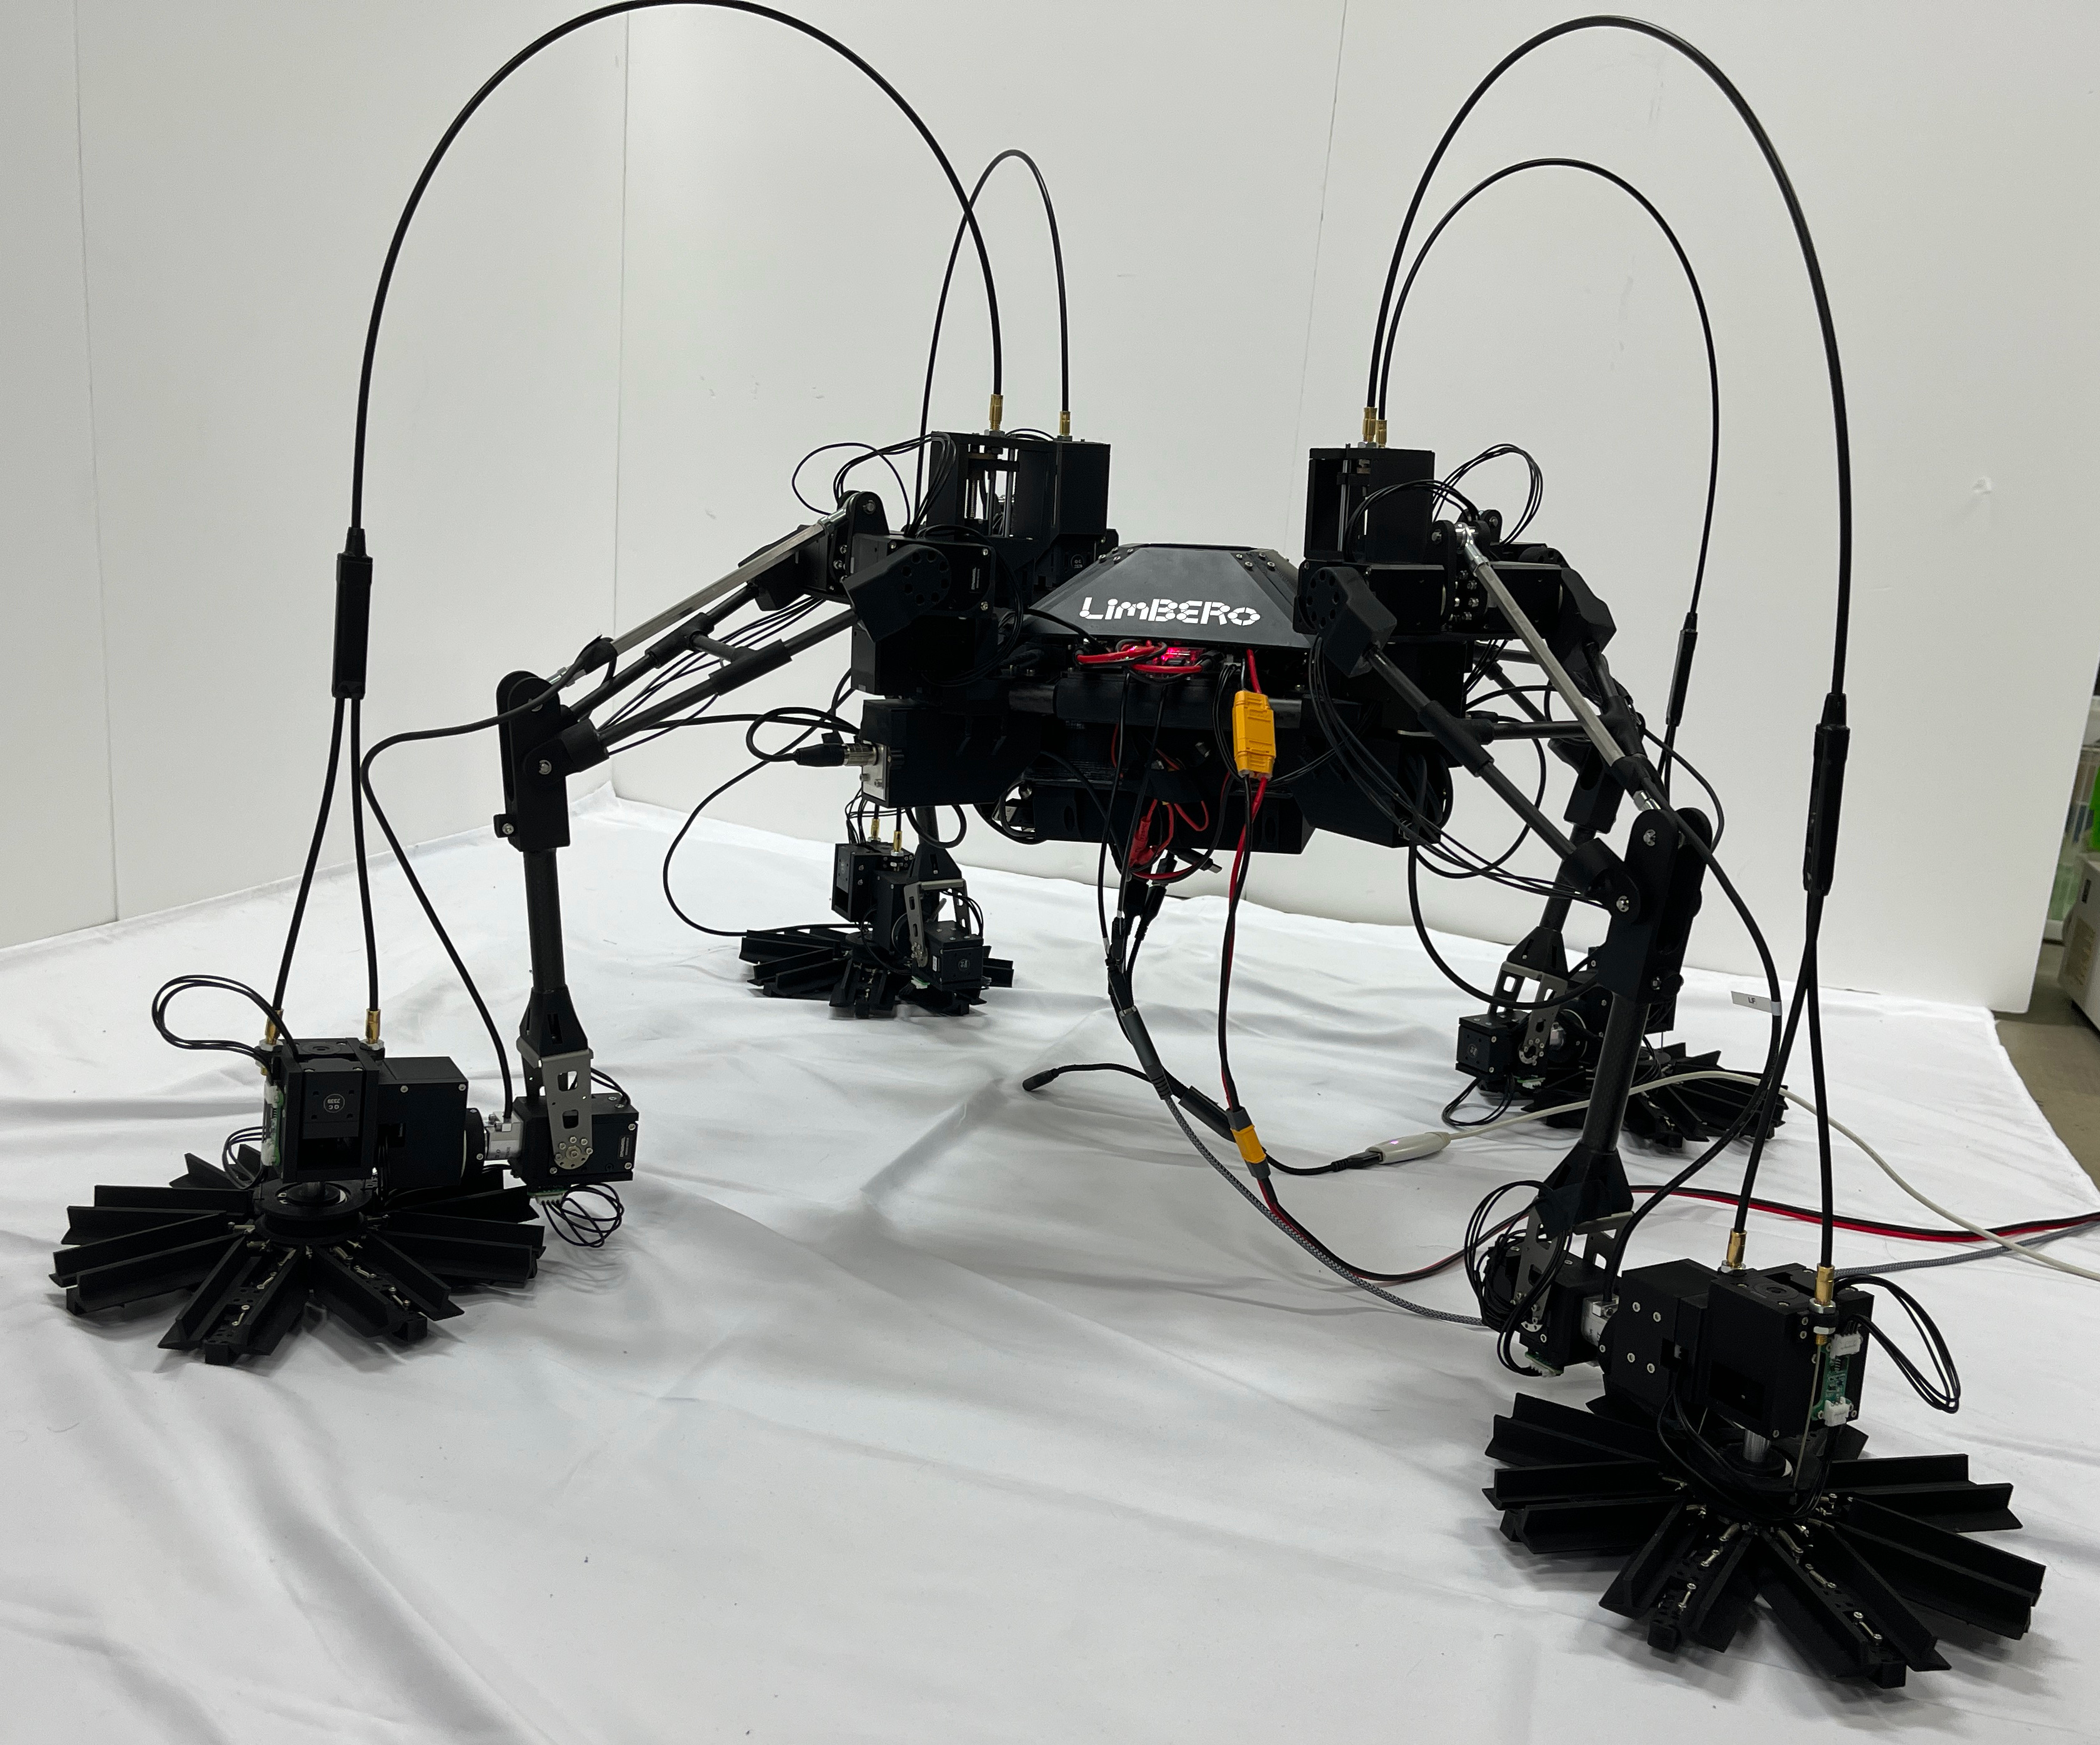
\includegraphics[width=0.4\textwidth]{Images/img_ch9/robot_gripper.png}} \quad 
    \subfloat[Wheel mode\label{fig:wheelv2}]{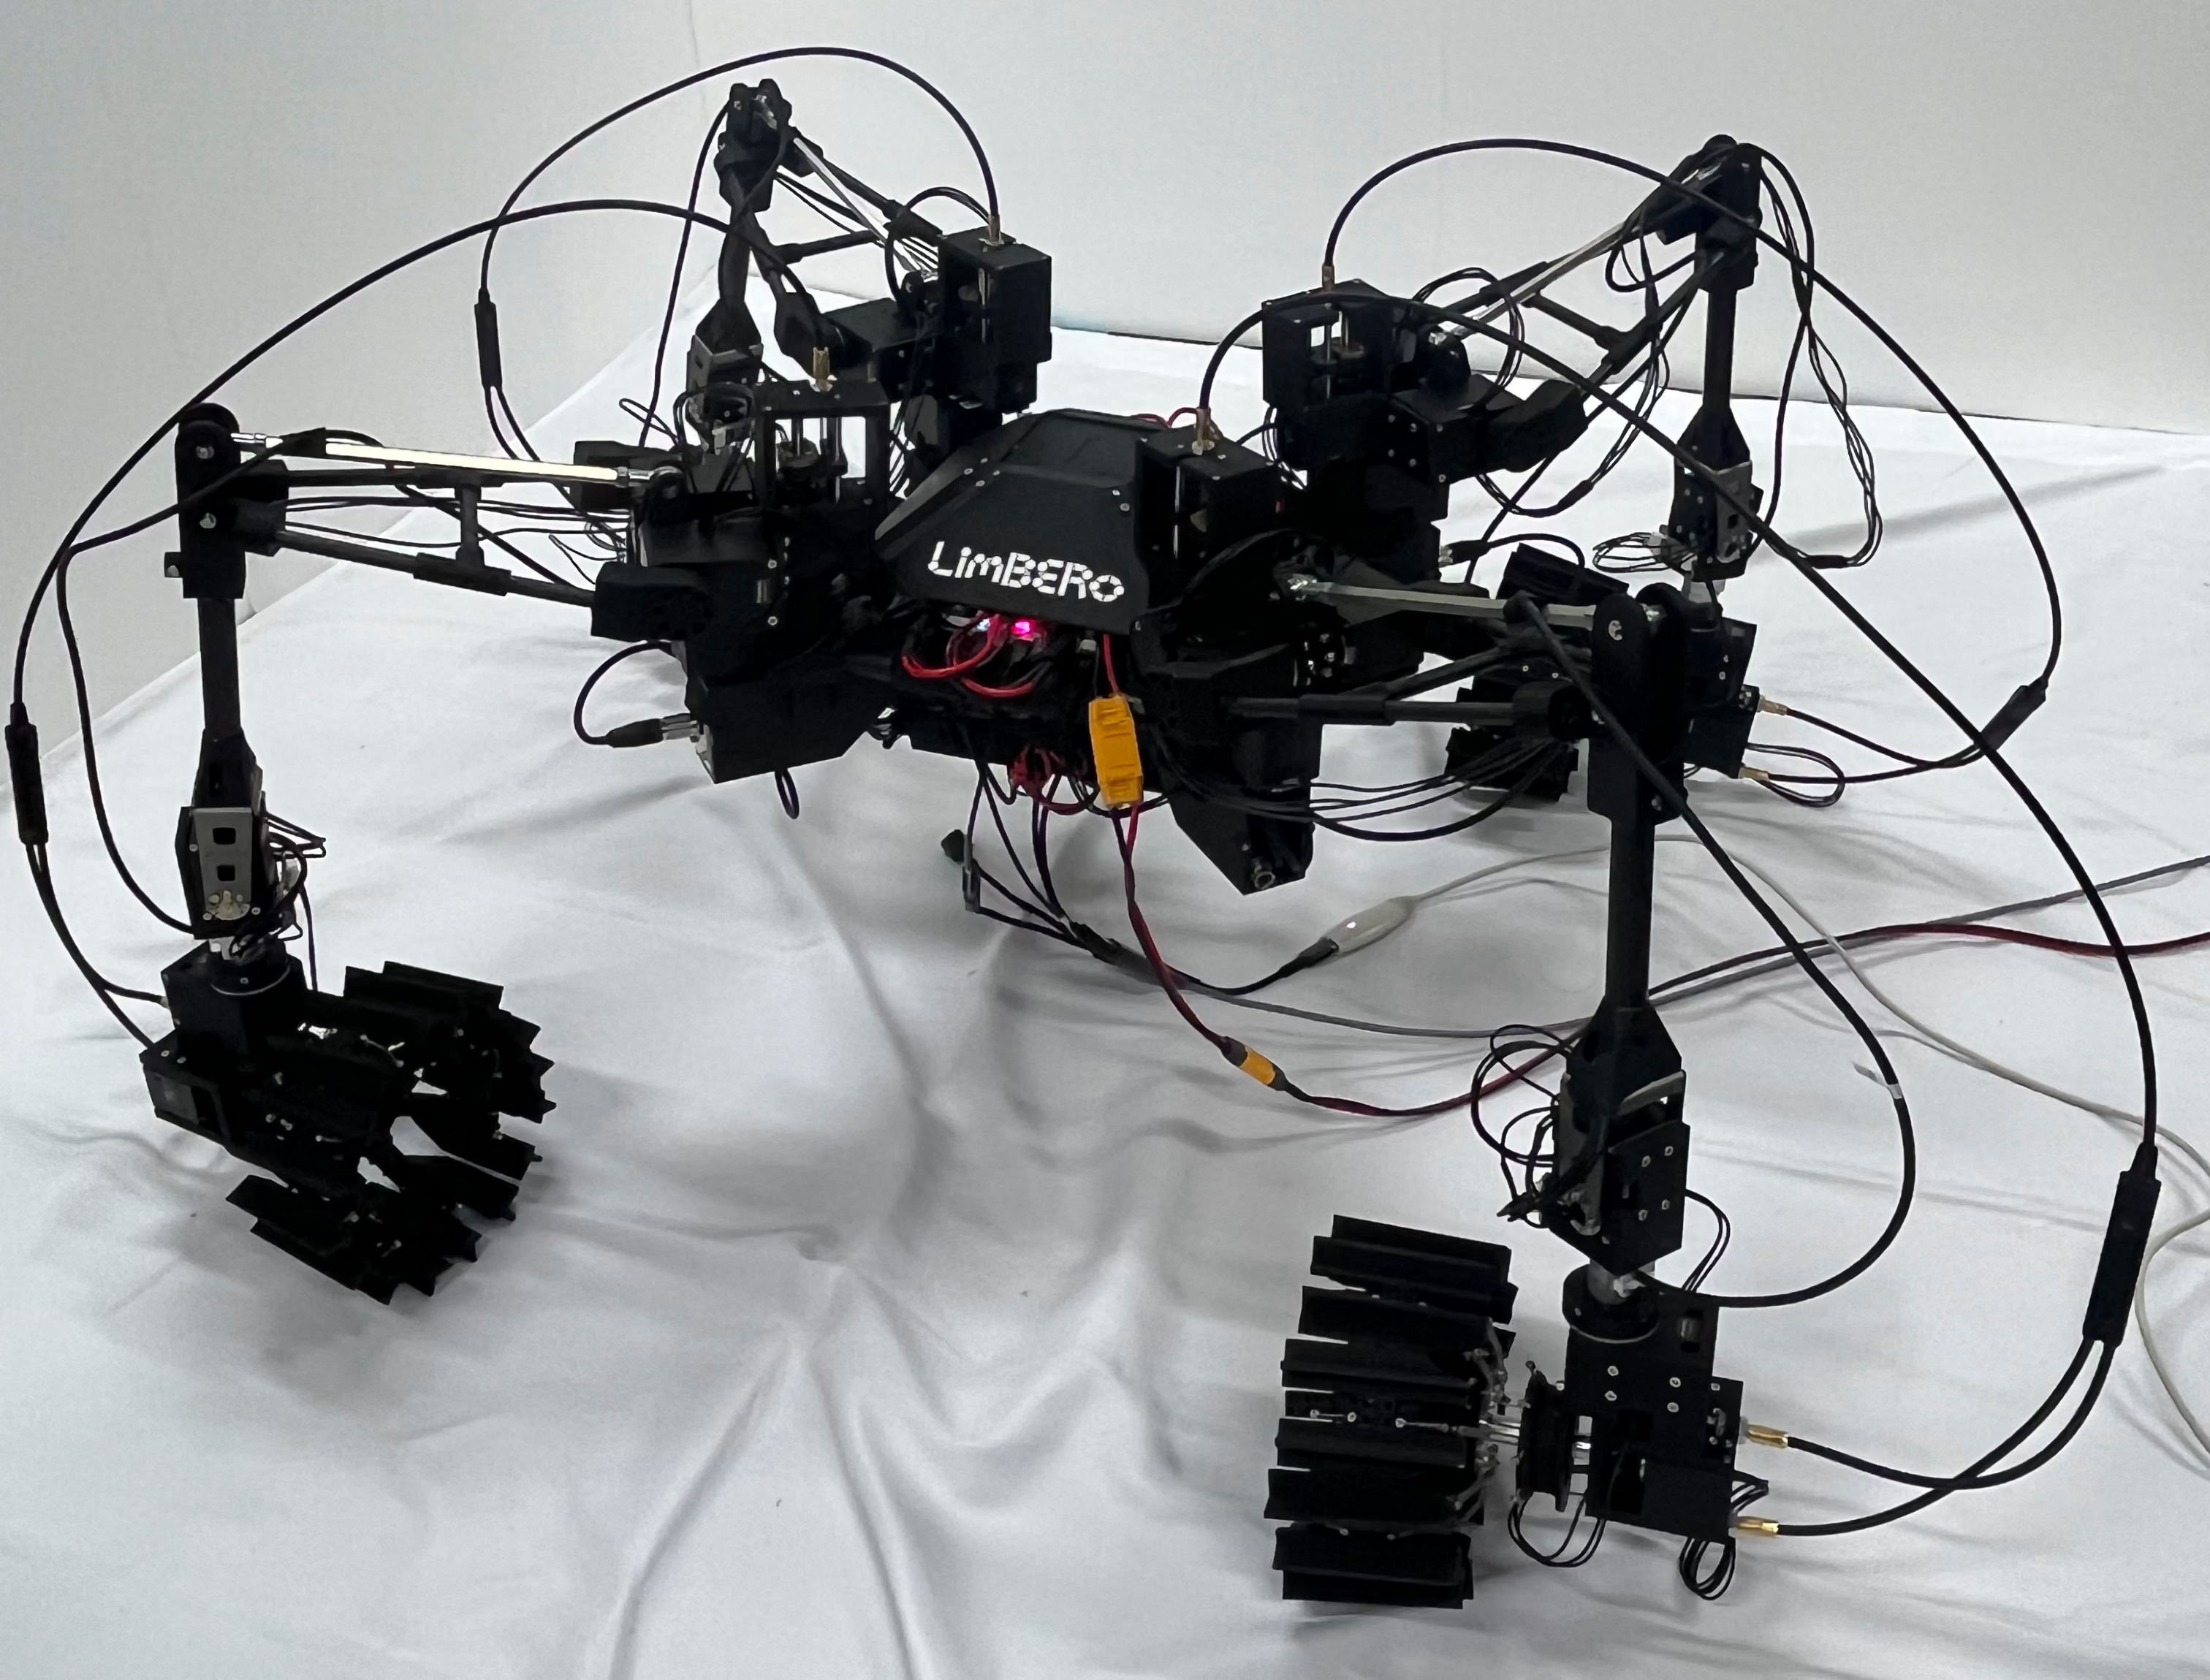
\includegraphics[width=0.4\textwidth]{Images/img_ch9/robot_wheel.png}} 
    \caption[LIMBERO-GRIEELv2]{LIMBERO-GRIEEL, new version}
    \label{fig:newrobot}
\end{figure}

In terms of \textbf{sensors}, some of the already available exteroceptive/proprioceptive sensors have not been used for this research, and are not discussed here. However, as already noticed, there is a need for feedback information on the GRIEEL finger's state, both for manipulation and transformation. Integrating a hardware solution such as a tether's tension sensor or some is a possible future development. Software solutions such as state estimators are not excluded. 

The contact state estimation is also an important aspect that will be considered in the future. During the experiments, the lack of limb-end contact feedback was a critical problem. To solve this issue, integrating sensors or state estimators is a fundamental next step for the full autonomy of the system, and for adapting the trajectory online.  

\subsection{Global Planning}
\label{sec:Decision}
The global planner is the higher-level component of the control architecture, and it is fundamental for enabling complete autonomy during robot missions.  
Also in semi-autonomous systems high-level planners are integrated, and an example is the Mars rover Perseverance. 

In classical mobile robots, this component is responsible for defining a feasible trajectory toward the goal for the navigation task. In manipulators instead, it computes an obstacle-free EE trajectory for the manipulation task.
When the trajectory is defined, a cost map of the environment is used, and the robot model can be integrated into a kinodynamic planning approach. 
Furthermore, when working with walking robots, a foothold has to be accurately chosen, and the same holds when climbing robots have to select grasping points, as discussed by K.Uno\cite{KentaroUnoPhD} and K.Takada\cite{LIMBEROTakadaThesis}.  

For a multimodal robot, as discussed in the final consideration of Chapter \ref{ch:chapter_five}, additional complexity is included in the high-level planning. The cost map has to be multilayered for the possible locomotion modality (walk, climb, drive), and the cost of transformation has to be included in the cost function. For this purpose, traversability analysis has to be integrated, and many alternative trajectories with different motion combinations will be compared.  

When object manipulation has to be performed, strategies used for manipulators will be integrated, and similar considerations hold in the autonomous grasping tasks during climbing, already under development. 

To conclude, the stable module transition algorithm defined previously is also part of a global planner, now some aspects already mentioned for future improvements are summarized.
\subsubsection{Transformation Algorithm Extension}

This research assumes that the module transition occurs in flat terrains and without relevant inertial effect (quasi-static motion). Under these assumptions, the stability is ensured by the SSM criterion. For this reason, the transformation algorithm discussed in chapter \ref{ch:chapter_five} adapts the motion sequence based on geometrical considerations only. As already mentioned, it is possible to integrate more reliable stability criteria for generic terrain characteristics, which are more common in unstructured environments. 

Therefore, considering the ZMP or GIA stability criterion to define the next base position, with the same approach of "look into future support state", is an interesting future development. However, with this extension, not only the future support polygon has to be estimated, but also the upcoming dynamical effect when the limb to transform is raised. 

\subsection{Local Planning}
\label{sec:Control}
Introduced in Chapter\ref{ch:chapter_two}, the local planner corresponds to the motion controller, so it is the component that defines the relationship from the desired state (and state feedback/estimation) to the control signal. 

In this research, most effort has been dedicated to the definition of a stable motion task in the autonomous adaptable transition algorithm, and a prototype controller has been implemented. When controlling the system with the IJC, a simple switching gain PI control is considered on the driving joint, and a unique cascade PPI for the other joints, with the tuning derived from an average model, but the multimodal aspect is not accounted for. 

In principle, the robustness of closed-loop PID control allows us to obtain satisfactory performances in both wheel and gripper modes when basic tasks are executed. 
However, when the potential of LIMBERO-GRIEEL is fully exploited, a fixed IKJC scheme for all the situations cannot ensure satisfactory performance. 
Now, some of the possible approaches are summarized, 

\subsubsection{Finite State Machine}
Similarly to the multimodal wheel-leg hexapod \cite{Hexapod_LegWheeled} represented in Fig.\ref{fig:hexapod_Legwheels}, to control and monitor the actual mode of
the robot, a finite state machine \textbf{for each limb} can be modeled, considering the states as: walking, climbing, driving, manipulating. Currently, only the wheel/gripper state is tracked, but additional internal knowledge is required to adapt the control logic. 

\subsubsection{Impedance control}
It is clear that in an unstructured environment, even if advanced vision systems are used, unexpected interactions with obstacles are inevitable, and the surface characteristic is not predictable. 
For this reason, controlling the limb tip position with the joint angles is unreliable. 

For this reason, integrating force-based control strategies is crucial to have a degree of adaptability to the terrain. 

The objective of impedance control is to establish a relationship between force and position, based on the desired apparent stiffness, dumping, or mass of the system\cite{ImpedanceControl}. This reduces the behavior to a mass-spring-dumper system with the desired dynamics, mitigating the effect of unexpected collisions and adapting to the ground reaction forces. 

An impedance control strategy is currently under development for LIMBERO, because of its importance when climbing motion is performed. Integrating this control strategy on LIMBERO-GRIEEL can enhance its performance both on wheel and gripper mode locomotion, enabling a control-based suspension behavior of the limbs. 

\subsubsection{Whole Body Controller and Extensions}
As the impedance control previously defined, this is a model-based strategy. 
While the impedance control is integrated into the system (after the task mapping to the desired state)  as part of the motion controller, the WBC defines a multilayered hierarchical structure. 
In particular, it is responsible for high-level planning, task-space mapping, optimization-based computation, and low-level control. This means that the impedance control can be part of a WBC, and an MPC is often integrated as an optimization component\cite{AnymalDocThesis}. 

The WBC control strategy is very promising, but it involves many modeling and optimization problems\cite{AnymalDocThesis}\cite{WBCFocchi}\cite{WBCQuadruped}. For this reason, its implementation on LIMBERO-GRIEEL is far in the future but considered as part of the next projects. 

 Extensions of the WBC strategies such as the one presented by O.Khatib \textit{et all} in \cite{KhatibConstrainedConsistentTaskOrientedWBC} integrate task and constraints with a system-oriented and natural solution, which is interesting for the future development of LIMBERO-GRIEEL. 

To conclude, in defining the optimization-based module of this hierarchical control strategy, integrating in the cost function the GIA for stability and the ATBVME for dexterity can enhance the system's performance. 

\subsubsection{Reinforcement Learning}
integrate
The research on Data-driven control algorithms is currently an active and evolving research area, and one of those control approaches is reinforcement learning\cite{RL_overview}\cite{InteligentControlMultiLegged}\cite{RobotSimulationRL}\cite{RL_wheelLegged}.   
With this control strategy, the robot learns how to achieve complex tasks by optimizing its behavior based on a training process, deriving at the end a probabilistic function that relates the desired task and current state to a control input. 

This approach is very promising for complex multidimensional systems such as LIMBERO-GRIEEL, and it is considered for future research to enable smooth locomotion in different modes and manipulation.



In conclusion, there are many approaches to control autonomous systems, especially for multimodal multifunctional robots like the one studied in this research. A possible future research project is the combination of different control solutions. 
For example, a finite state machine controller, where each state is a hierarchical controller, and the cost function of the optimization layer considers different performance indices according to the locomotion mode, including the dexterity index to use an ellipsoid tracking optimal approach\cite{EllipsoidTracking}. 

\subsection{Conclusion}
\label{sec:conclusion}

The potential of this cutting-edge robotic system has been commented on several times in this research, but also its complexity. 
Based on the preceding discussion, a potential roadmap toward full system autonomy is illustrated in Fig.\ref{fig:roadmap}. These components are interconnected in the multilayered structure, and their development requires expertise and novel solutions in robotics research.

\begin{figure}[H]
    \centering
    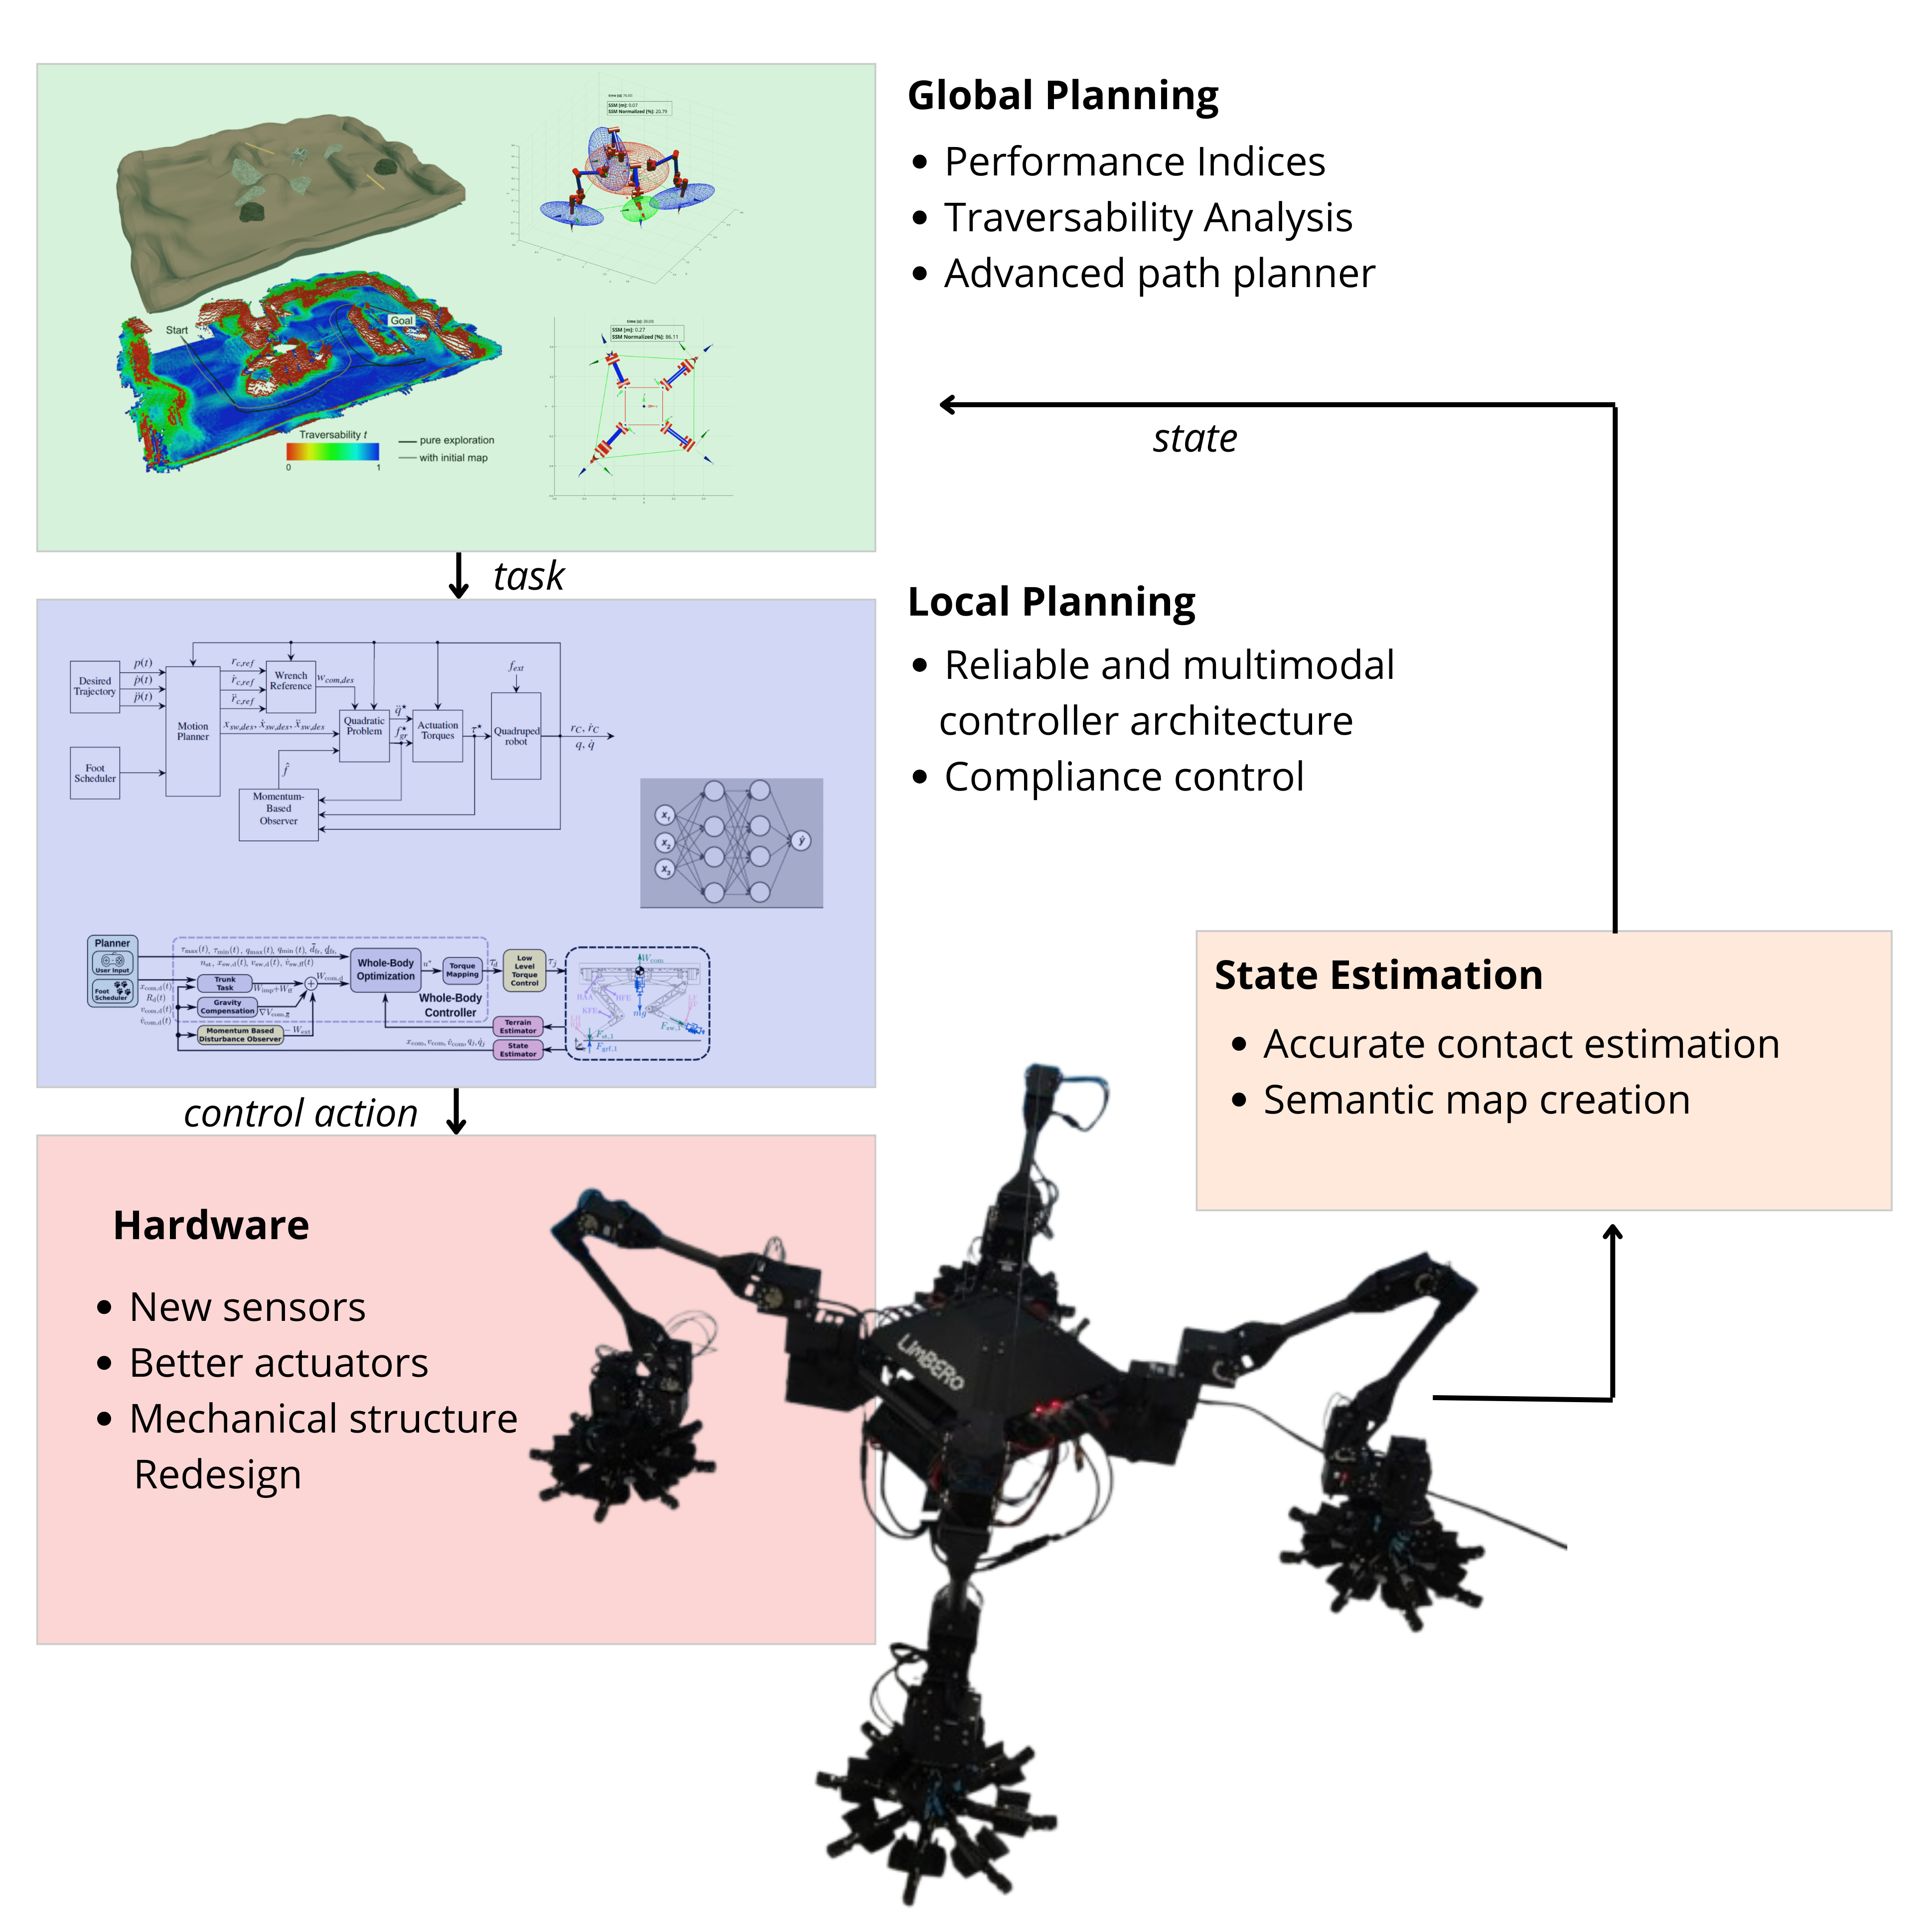
\includegraphics[width=0.65\textwidth]{Images/img_ch9/roadmap.png}
    \caption{Future development roadmap}
    \label{fig:roadmap}
\end{figure}


